\documentclass{school-22.211-notes}
\date{May 12, 2012}

\begin{document}
\maketitle


%%%%%%%%%%%%%%%%%%%%%%%%%%%%%%%%%%
\lecture{Adjoint Fluxes, Perturbation Theory}\label{adjoint-fluxes}
Perturbation theory provides us a pretty accurate prediction of reactivity without knowning $\delta \psi$. There is no reactivity associated with a space and a time (it has a reactivity contribution). Reactivity is always integrated over the entier system because of the denominator. 

\topic{Adjoint Fluxes for Critical Reactor Systems}
We express the transport of diffusion equation in operator notation, 
\eqn{ A\psi &= \frac{1}{k} M \psi &A^*\psi^* &= \frac{1}{k^*} M^* \psi^*  }
We multiply the forward equation by adjoint flux, multiply the adjoint equation by real flux, subtract the two and integrate over the phase space to get, 
\eqn{ \expect{ \psi^*, A\psi}  - \expect{\psi, A^* \psi^*} - \frac{1}{k} \expect{ \psi^*, M \psi} + \frac{1}{k^*} \expect{ \psi, M^* \psi^*} &= 0 }
But recalling the definition of the adjoint operating on any operator $f$, 
\eqn{ \expect{ \psi^*, f\psi} &= \expect{\psi, f^* \psi^*} }
Consequently, 
\eqn{ \expect{ \frac{1}{k} - \frac{1}{k^*} } \expect{ \psi^*, M \psi} &= 0 }
The fundamental mode solution, which is the one we are interested in, has everywhere positive real and adjoint fluxes, and since the fission operator is an everywhere positive operator, we find that the real and adjoint eigenvalus must be identical,
\eqn{ k^* &= k }

\clearpage
\topic{First Order Perturbation Theory (FOP)}
In this section we evaluate the Rayleigh quotient $\displaystyle \lambda[\phi, \phi^*] = \frac{\expect{\phi^*, A \phi}}{\phi^*, F \phi}$ for a critical reactor eigenvalue problem described by the transport and adjoint equations. 

\begin{enumerate}
\item We start from an unperturbed system 
\eqn{ A_0 \psi_0 &= \frac{1}{k_0} M_0 \psi_0 &A_0^*\psi_0^* &= \frac{1}{k_0^*} M^* \psi_0^*  }

\item The perturbed system has operators, 
\eqn{ A &= A_0 + \delta A   &M &=M_0 + \delta M  &\psi &=\psi_0 + \delta \psi &k&=k_0+\delta k}
and approximate the perturbed system with, 
\eqn{ (A_0 + \delta A) (\psi_0 + \delta \psi) &= \frac{1}{k_0+\delta k} (M_0 + \delta M) (\psi_0 + \delta \psi) \label{perturbed-sys}}
We first expand the $\keff$ term, 
\eqn{ \frac{1}{k_0+\delta k} = \frac{1}{k_0} \frac{1}{1 + \delta k /k_0} = \frac{1}{k_0} - \frac{\delta k}{k_0^2} + O(\delta k^2)  }
Plug back into Eq.~\ref{perturbed-sys}, 
\begin{align}
(A_0 + \delta A) (\psi_0 + \delta \psi) &= \left( \frac{1}{k_0} - \frac{\delta k}{k_0^2}  \right) (M_0 + \delta M) (\psi_0 + \delta \psi) \\
A_0 \psi_0 + A_0 \delta \psi + \delta A \psi_0 &= \frac{1}{k_0} M_0 \psi_0 + \frac{1}{k_0} M_0 \delta \psi + \frac{1}{k_0} \delta M \psi_0 - \frac{\delta k}{k_0^2} M_0 \psi_0 + O(\delta^2)  
\end{align}
\eqn{ \overbrace{ \left( A_0 - \frac{1}{k_0} M_0 \right) \psi_0}^{\to 0} + \left( A_0 - \frac{1}{k_0} M_0 \right) \delta \psi + \left( \delta A - \frac{1}{k_0} \delta M \right) \psi_0 &= - \frac{\delta k}{k_0^2} M_0  \psi_0 + O(\delta^2)  }
\eqn{ -\frac{\delta k}{k_0^2} M_0 \psi_0 &= \left( \delta A - \frac{1}{k_0} \delta M \right) \psi_0 + \left( A_0 - \frac{1}{k_0} M_0 \right) \delta \psi + O (\delta^2) }
Multiply by $\psi^*$ and integrating over phase space, 
\eqn{ - \frac{\delta k}{k_0^2} \expect{ \psi^*, M_0 \psi_0} &= \expect{ \psi^*, \left( \delta A - \frac{1}{k_0} \delta M \right) \psi_0 } + \overbrace{ \expect{\psi^*, \left( A_0 - \frac{1}{k_0} M_0 \right) \delta \psi} }^{\textcircled{1}} + O(\delta^2) \label{perturbed-sys2} }

\item We use the definition of adjoint operator for any operator, 
\eqn{ \textcircled{1} =  \expect{\psi_0^*, \left( A_0 - \frac{1}{k_0} M_0 \right) \delta \psi} =  \expect{\delta \psi, \left( A_0^* - \frac{1}{k_0^*} M_0^* \right) \psi_0^*} = 0 }
Then Eq.~\ref{perturbed-sys2} becomes, 
\eqn{ - \frac{\delta k}{k_0^2} &= \frac{\expect{ \psi_0^*, \left( \delta A - \frac{1}{k_0} \delta M \right) \psi_0 }}{\expect{ \psi_0^*, M_0 \psi_0} } + O(\delta^2) \label{perturbed-sys3} }
Notice that, 
\begin{itemize}
 \item There are only second order errors in reactivity, because the term multiplying $\delta \psi$ is zero, hence the first order error vanishes in the reactivity expression. 
 \item Thus Eq.~\ref{perturbed-sys3} is clearly much more accurate than the 1st order accurate expression we had before we multiply by $\psi_0^*$ and integrate,
   \eqn{ - \frac{\delta k}{k_0^2} &= \frac{ \left(\delta A - \frac{1}{k_0} \delta M\right) \psi_0 + \left( A_0 - \frac{1}{k_0} M_0 \right) \delta \psi}{M_0 \psi_0} + O (\delta^2) }
\end{itemize}

 \item Finally making use of the definition of reactivity, 
   \eqn{ \rho &= \frac{k-1}{k} &\Rightarrow \rho - \rho_0 &= \frac{k - 1}{k} - \frac{k_0-1}{k_0} = \frac{\delta k}{k k_0} &\delta \rho &= \frac{\delta k}{k_0^2} + O(\delta k^2) }
   One obtains the first order perturbation (FOP) expression for reactivity, 
   \eqn{ \boxed{\delta \rho \approx \frac{\expect{\psi_0^*, \left( \frac{1}{k_0} \delta M - \delta A \right) \psi_0 }}{\expect{\psi_0^*, M_0 \psi_0}}  } }
\end{enumerate}
Interpretations of the $\delta \rho$ equation, 
\begin{itemize}
\item One can evaluate reactivity resulting from any changes in operator, e.g., fuel temperature, coolant density, boron concentration, by simply evaluating delta cross sections convoluted on unperturbed real and adjoint fluxes. 

\item Because of the linearility of the first-order perturbation theory, we can super-impose: 
  \begin{itemize}
  \item reactivity contributions from perturbations in different spatial regions;
  \item reactivity effects from perturbations in different phenomenon, e.g., coolant density and temperature. 
  \end{itemize}

\item Each reactivity perturbation can be computed without need for solving for perturbed spatial flux distributions. 
\end{itemize}

\clearpage
\topic{Relating Adjoint Flux to Neutron Population}
We consider the same problem two ways.
\begin{enumerate}
\item From the point kinetics that the neutron population is given by, 
\begin{align}
  \ddt N(t) &= \frac{\rho(t) - \Sum_i \beta_i}{\Lambda} N(t) + \Sum_i \lambda_i C_i(t) + Q \\
  \ddt C_i (t) &= \frac{\beta_i}{\Lambda} N(t) - \lambda_i C_i (t)
\end{align}
For criticality $\rho=0$, precursor populations are not changing $\frac{\beta_i}{\Lambda}N(t) = \lambda_i C_i(t)$, hence the RHS of $\ddt N(t)$ only have the source term left, 
\eqn{ \ddt N(t) = Q}
That is, for a constant external source $Q$ (unit: neutrons/s), neutron polulation grows linearly in time with $Q$,
\eqn{  N(t) = N_0 + Q(t-t_0)}

\item Now consider introducing $Q$ neutrons: at time zero at position, energy, and direction $(\vecr, \Omegahat, E)$ then
\eqn{ \ddt N(t) &= Q  \delta (t - t_0) \Rightarrow N(\infty) = N_0 + Q \cdot X} 
Or 
\eqn{ \ddt N(t) &= Q \delta (t - t_0) \Rightarrow N(\infty) = N_0 + Q \psi^* (\vecr, \Omegahat, E)  }
\end{enumerate}

Combining the two methods, we get
\eqn{  \Aboxed{\frac{N(\infty) - N_0}{Q} &= \psi^* (\vecr, \Omegahat, E)  } }
\hi{The adjoint flux is defined as the asymptotic increase in total neutron population of a critical reactor for a neutron introduced in a phase space (position $r$, direction $\omega$, and energy $E$).} The adjoint is only defined for what reaction that we are interested in: in a critical reactor, that is neutron population; in a subcritical system, like the one in detector, then it is whatever purpose, like detector response, that we are interested in. 


\clearpage
\topic{Multi-Group Real and Adjoint Flux Equations}
Hebert states that the general rules for creating the adjoint of an operator are (p.77): 
\begin{enumerate}
\item Transpose the matrix operators. 
\item Change the sign of odd-parity differential operators. E.g., $\vec{\Omega} \cdot \gradient \phi \to - \vec{\Omega} \cdot \gradient \phi^*$. 
\item Interchange the arguments of the kernels of integral operators. 
\end{enumerate}

\begin{align}
 -\gradient D_g (\vecr) \gradient \phi_g(\vecr) + \Sigma_{tg} (\vecr) \phi_g(\vecr) &= \chi_g \Sum_{g'=1}^G \nu \Sigma_{fg'} (\vecr) \phi_{g'}(\vecr) + \Sum_{g'=1}^G \Sigma_{sg'\to g} (\vecr) \phi_{g'}(\vecr) \\
 -\gradient D_g (\vecr) \gradient \phi_g^* (\vecr) + \Sigma_{tg} (\vecr) \phi_g^* (\vecr) &= \nu \Sigma_{fg} (\vecr)\Sum_{g'=1}^G \chi_{g'} \phi_{g'}^* (\vecr) + \Sum_{g'=1}^G \Sigma_{sg\to g'} (\vecr) \phi_{g'}^*(\vecr)
\end{align}
For two group, infinite medium case, with effective downscatter only, 
\begin{align}
\left[ \begin{array}{cc}
\Sigma_{a1} + \Sigma_{12} - \frac{1}{\kinf} \nu \Sigma_{f1} & - \frac{1}{\kinf} \nu \Sigma_{f2} \\
- \Sigma_{12} & \Sigma_{a2} \end{array} \right] 
\left[ \begin{array}{c}
\phi_1 \\ \phi_2 \end{array} \right] &= 0  
&\frac{\phi_2}{\phi_1} &= \frac{\Sigma_{12}}{\Sigma_{a2}}   \\
\left[ \begin{array}{cc}
\Sigma_{a1} + \Sigma_{12} - \frac{1}{\kinf^*} \nu \Sigma_{f1} & - \Sigma_{12} \\
- \frac{1}{\kinf^*} \nu \Sigma_{f2} & \Sigma_{a2} \end{array} \right] 
\left[ \begin{array}{c}
\phi_1^* \\ \phi_2^* \end{array} \right] &= 0  
&\frac{\phi_2^*}{\phi_1^*} &= \frac{\frac{1}{\kinf^*} \nu \Sigma_{f2}}{\Sigma_{a2}}  
\end{align}
where 
\eqn{ \kinf^* = \kinf = \frac{\nu \Sigma_{f1}  + \nu \Sigma_{f2} \frac{\Sigma_{12}}{\Sigma_{a2}} }{\Sigma_{a1} + \Sigma_{12}} } 
The above expressions show that knowing cross sections, we know $\kinf$, hence we know $\kinf^* = \kinf$, then we can solve for $\frac{\phi_2^*}{\phi_1^*}$. 
\end{document}

\begin{figure}[ht]
  \centering
  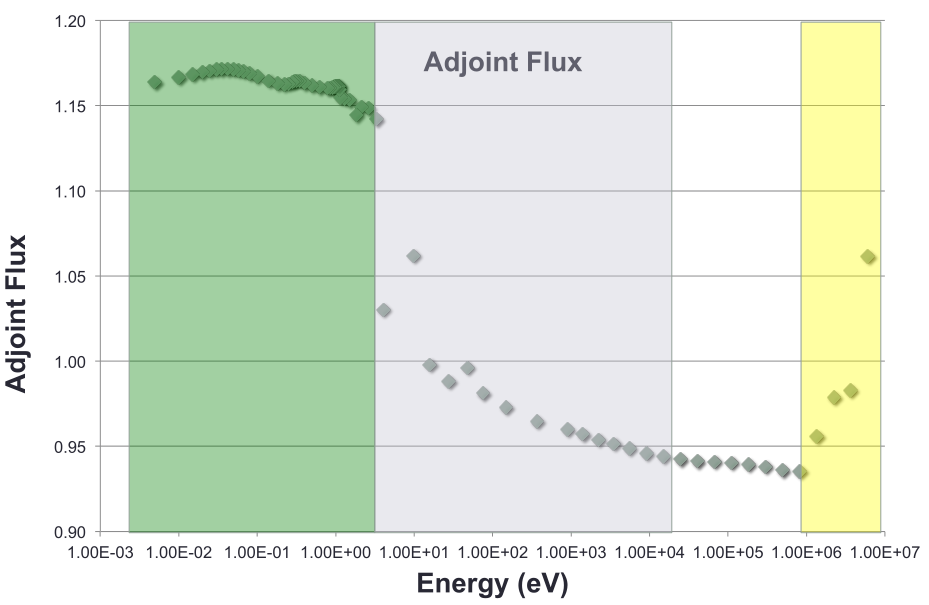
\includegraphics[width=5in]{images/methd/adjoint-spec.png}
  \caption{PWR Lattice Adjoint Spectrum}
\end{figure}
We are also interested in adjoint weighted reactivity expression as in Fig.~\ref{adjoint-weighted-reactivity}. Recall that PKE assumes flux shape does not change with respect with time. We use adjoint flux weighted PKE to account for the flux change. \hi{$\beta$ is very sensitive to adjoint flux.} 

\begin{figure}[ht]
  \centering
  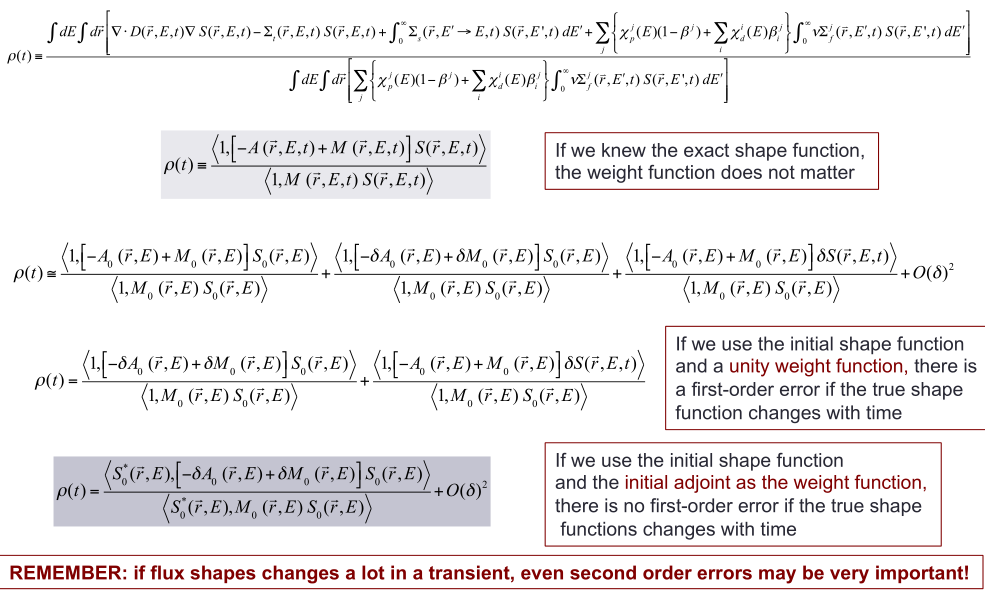
\includegraphics[width=5.5in]{images/methd/adjoint-weighted-reactivity.png}
  \\
  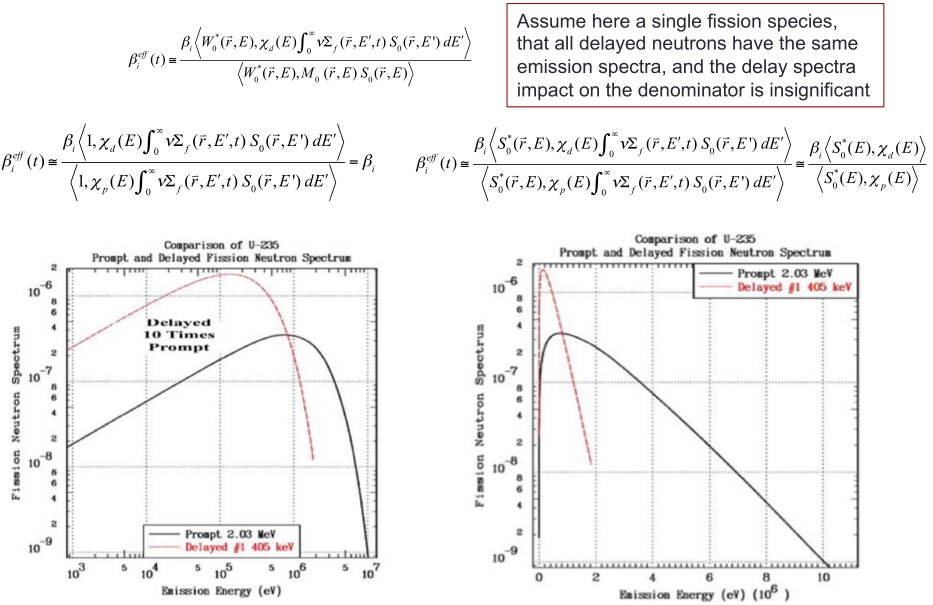
\includegraphics[width=5.5in]{images/methd/adjoint-weighted-reactivity-2.png}
  \caption{Adjoint Weighted Reactivity} \label{adjoint-weighted-reactivity}
\end{figure}

\begin{figure}[ht]
  \centering
  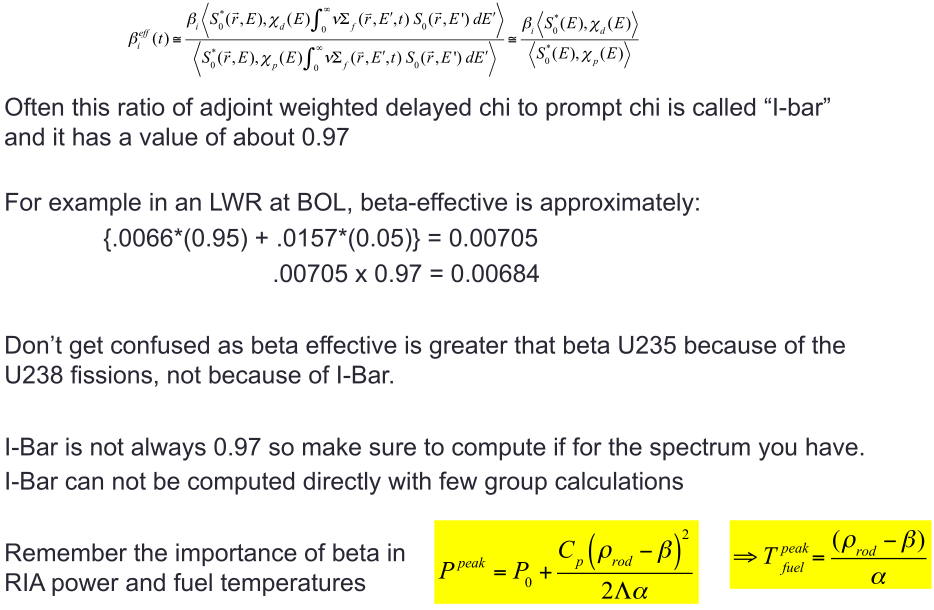
\includegraphics[width=5in]{images/methd/beta-effective.png}
  \caption{LWR Beta Effective and I-bar}
\end{figure}

\end{document}
